\scanpage{95}
\figure{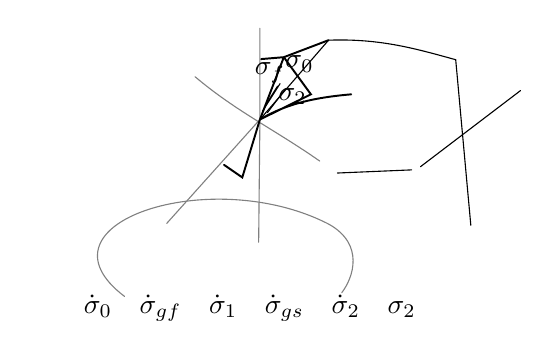
\begin{tikzpicture}[x=.008cm,y=-.008cm,line cap=round]
\draw[gray] (420,490)--(568,325)--(568,180) (568,325)--(566,520) (465,257)..controls(530,312)and(590,340)..(663,391);
\draw (568,325)--(677,199)..controls(760,196)and(817,213)..(879,230)--(903,493) (823,400)--(982,279) (691,410)--(809,405);
\draw[line width=.7pt] (511,397)--(540,417)--(568,325)--(606,226)--(677,199) (568,325)--(649,285)--(606,226)--(570,229) (568,325)..controls(610,300)and(655,290)..(713,285);
\draw (572,312)--(600,268) (580,314)--(609,276) (579,299)--(596,272);
\node at (584,251) {$\sigma_f$};\node at (631,237) {$\sigma_0$};\node at (620,288) {$\sigma_2$};
\draw[gray] (353,606)..controls(200,490)and(490,395)..(677,491)..controls(735,523)and(716,577)..(698,600);
\node[anchor=north] at (552,588) {$\dot\sigma_0\quad\dot\sigma_{\deleted{\unsure{g}}\inserted{f}}\quad\dot\sigma_1\quad\dot\sigma_{\deleted{\unsure{g}}\inserted{s}}\quad\dot\sigma_2\quad\deleted{\unsure{\sigma_2}}$};
\end{tikzpicture}}
\figure{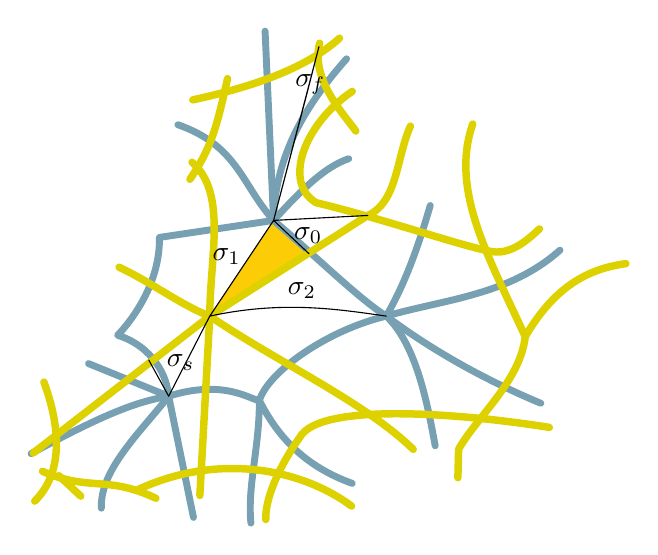
\begin{tikzpicture}[x=.009cm,y=-.009cm,line cap=round,line join=round]
\fill[yellow!65!orange] (1240,525)--(1330,390)--(1380,437)--cycle;
\draw[cyan!35!gray,line width=2.5pt] (1318,123)--(1330,390)..controls(1400,450)and(1450,500)..(1489,525)..controls(1530,564)and(1546,642)..(1558,708);
\draw[cyan!35!gray,line width=2.5pt] (1195,255)..controls(1280,285)and(1285,340)..(1330,390)..controls(1332,294)and(1380,222)..(1433,162);
\draw[cyan!35!gray,line width=2.5pt] (1330,390)..controls(1370,346)and(1403,314)..(1436,303);
\draw[cyan!35!gray,line width=2.5pt] (1330,390)--(1169,414)..controls(1170,478)and(1131,530)..(1110,552)..controls(1160,568)and(1180,610)..(1182,638)--(1217,809);
\draw[cyan!35!gray,line width=2.5pt] (988,719)..controls(1100,658)and(1142,645)..(1182,638)..controls(1261,613)and(1299,644)..(1310,644)..controls(1310,712)and(1293,763)..(1298,817);
\draw[cyan!35!gray,line width=2.5pt] (1087,796)..controls(1085,742)and(1141,690)..(1182,638)--(1069,592);
\draw[cyan!35!gray,line width=2.5pt] (1489,525)..controls(1405,545)and(1322,604)..(1310,644)..controls(1337,698)and(1377,738)..(1441,761);
\draw[cyan!35!gray,line width=2.5pt] (1489,525)..controls(1518,475)and(1537,417)..(1551,369);
\draw[cyan!35!gray,line width=2.5pt] (1489,525)..controls(1572,501)and(1662,496)..(1734,432);
\draw[cyan!35!gray,line width=2.5pt] (1489,525)..controls(1557,576)and(1633,617)..(1707,648);
\draw[yellow!70!olive,line width=2.7pt] (1216,220)..controls(1298,202)and(1374,177)..(1423,133);
\draw[yellow!70!olive,line width=2.7pt] (1395,140)..controls(1382,192)and(1430,241)..(1446,264);
\draw[yellow!70!olive,line width=2.7pt] (1441,208)..controls(1374,253)and(1342,336)..(1390,365)..controls(1486,388)and(1594,426)..(1638,434)..controls(1667,439)and(1693,413)..(1705,402);
\draw[yellow!70!olive,line width=2.7pt] (1265,190)..controls(1249,263)and(1241,289)..(1212,332);
\draw[yellow!70!olive,line width=2.7pt] (1215,308)..controls(1265,351)and(1240,442)..(1240,525)--(1226,778);
\draw[yellow!70!olive,line width=2.7pt] (1611,254)..controls(1578,348)and(1635,444)..(1685,554)..controls(1727,482)and(1775,458)..(1827,451);
\draw[yellow!70!olive,line width=2.7pt] (1685,554)..controls(1678,617)and(1615,669)..(1591,713)--(1590,753);
\draw[yellow!70!olive,line width=2.7pt] (1523,257)..controls(1503,302)and(1505,364)..(1463,383)--(1240,525)--(991,718);
\draw[yellow!70!olive,line width=2.7pt] (1112,456)..controls(1157,477)and(1202,511)..(1240,525)..controls(1332,588)and(1460,647)..(1527,713);
\draw[yellow!70!olive,line width=2.7pt] (1719,682)..controls(1587,661)and(1394,647)..(1367,696)..controls(1335,741)and(1318,785)..(1319,812);
\draw[yellow!70!olive,line width=2.7pt] (1006,618)..controls(1030,683)and(1033,747)..(993,786);
\draw[yellow!70!olive,line width=2.7pt] (1004,744)..controls(1071,773)and(1094,749)..(1164,782);
\draw[yellow!70!olive,line width=2.7pt] (1136,771)..controls(1252,716)and(1370,741)..(1440,793);
\draw[yellow!70!olive,line width=2.7pt] (1027,750)--(1058,779);
\draw (1330,390)--(1394,145)--(1375,219)--(1330,390)--(1463,383) (1240,525)--(1330,390)--(1380,437) (1240,525)..controls(1342,503)and(1419,515)..(1489,525) (1240,525)--(1182,638)--(1154,587);
\node at (1382,198) {$\sigma_f$};\node at (1379,411) {$\sigma_0$};\node at (1264,441) {$\sigma_1$};\node at (1370,489) {$\sigma_2$};\node at (1199,590) {$\sigma_s$};
\end{tikzpicture}}
\figure{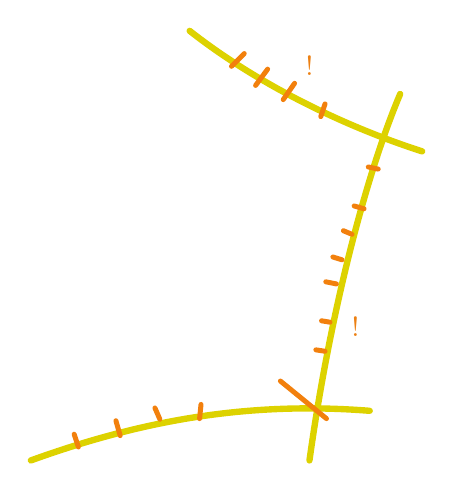
\begin{tikzpicture}[x=.009cm,y=-.009cm,line cap=round]
\draw[yellow!70!olive,line width=2.3pt] (2321,61)..controls(2415,135)and(2537,195)..(2649,231) (2618,150)..controls(2572,258)and(2520,452)..(2490,667) (2097,667)..controls(2260,608)and(2410,584)..(2575,597);
\draw[orange!80!brown,line width=1.8pt] (2380,111)--(2398,93) (2414,138)--(2431,115) (2453,158)--(2469,135) (2506,182)--(2512,164) (2573,253)--(2587,256) (2553,308)--(2567,312) (2538,343)--(2550,348) (2523,380)--(2536,384) (2513,415)--(2528,418) (2507,470)--(2519,472) (2499,511)--(2512,513) (2449,555)--(2514,608) (2158,630)--(2164,648) (2217,611)--(2223,632) (2272,593)--(2279,609) (2337,588)--(2335,608);
\node[text=orange!70!brown] at (2490,111) {$\unsure{!}$};\node[text=orange!70!brown] at (2555,479) {$!$};
\end{tikzpicture}}

Une carte dont les sommets
\uline{et} les faces sont d'ordre
pair, donne naissance à
une suite circulaire de
cinq involutions $2$ à $2$
commutantes
\[
\sigma_0\ \sigma_f\ \sigma_1\ \sigma_s\ \sigma_2\ [\sigma_0\ldots]
\]
donc à une carte pentagonale
\unsure{foncière|pondérée}, dont tous les
sommets sont d'ordre
deux ou quatre. Je n'arrive
pas bien à visualiser cette
dernière carte en termes de
la carte initiale....
\figure{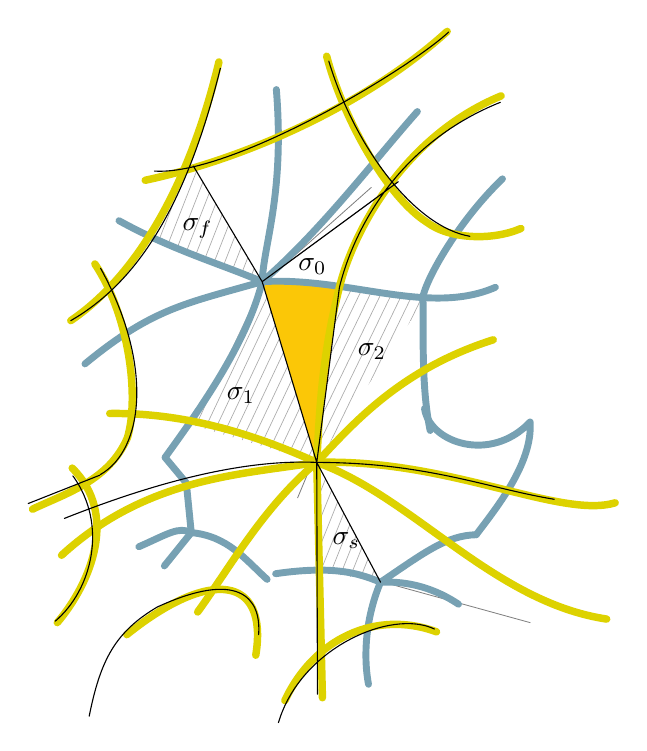
\begin{tikzpicture}[x=.009cm,y=-.009cm,line cap=round,line join=round]
\fill[yellow!60!orange] (1608,1143)--(1717,1151)--(1685,1398)--cycle;
\begin{scope}\clip (1511,980)--(1608,1143)--(1454,1086)--cycle;\foreach \k in {1410,1425,...,1635}\draw[gray!65,line width=.25pt](\k,1180)--++(90,-230);\end{scope}
\begin{scope}\clip (1608,1143)--(1505,1344)--(1685,1398)--cycle;\foreach \k in {1425,1440,...,1710}\draw[gray!65,line width=.25pt](\k,1440)--++(170,-360);\end{scope}
\begin{scope}\clip (1717,1151)--(1835,1172)--(1685,1398)--cycle;\foreach \k in {1580,1595,...,1865}\draw[gray!65,line width=.25pt](\k,1440)--++(160,-330);\end{scope}
\begin{scope}\clip (1685,1398)--(1775,1567)--(1685,1551)--cycle;\foreach \k in {1630,1645,...,1800}\draw[gray!65,line width=.25pt](\k,1590)--++(80,-200);\end{scope}
\draw[gray,line width=.3pt] (1608,1143)--(1800,1002) (1610,1145)--(1762,1010) (1678,1400)--(1658,1448) (1768,1564)--(1986,1624);
\draw[cyan!35!gray,line width=2.5pt] (1628,872)..controls(1640,1020)and(1610,1090)..(1608,1143)..controls(1586,1232)and(1515,1330)..(1471,1391)--(1501,1427)--(1508,1497)--(1470,1544);
\draw[cyan!35!gray,line width=2.5pt] (1358,1259)..controls(1454,1180)and(1500,1174)..(1608,1143)..controls(1691,1071)and(1766,972)..(1827,903);
\draw[cyan!35!gray,line width=2.5pt] (1406,1057)..controls(1480,1098)and(1552,1119)..(1608,1143)..controls(1730,1136)and(1843,1192)..(1937,1151);
\draw[cyan!35!gray,line width=2.5pt] (1947,998)..controls(1877,1065)and(1828,1160)..(1835,1172)..controls(1835,1238)and(1834,1300)..(1845,1353);
\draw[cyan!35!gray,line width=2.5pt] (1837,1322)..controls(1844,1370)and(1930,1400)..(1986,1341)..controls(1990,1400)and(1936,1465)..(1910,1500);
\draw[cyan!35!gray,line width=2.5pt] (1434,1517)..controls(1475,1499)and(1490,1488)..(1508,1497)..controls(1560,1502)and(1584,1535)..(1615,1563);
\draw[cyan!35!gray,line width=2.5pt] (1627,1555)..controls(1715,1542)and(1750,1557)..(1775,1567)..controls(1837,1525)and(1868,1501)..(1910,1500);
\draw[cyan!35!gray,line width=2.5pt] (1775,1567)..controls(1815,1565)and(1852,1576)..(1885,1598) (1775,1567)..controls(1755,1614)and(1750,1668)..(1758,1711);
\draw[yellow!70!olive,line width=2.7pt] (1547,833)..controls(1500,1029)and(1418,1144)..(1338,1198);
\draw[yellow!70!olive,line width=2.7pt] (1443,1000)..controls(1592,968)and(1759,890)..(1869,790);
\draw[yellow!70!olive,line width=2.7pt] (1699,825)..controls(1723,915)and(1785,1024)..(1840,1059)..controls(1873,1084)and(1934,1085)..(1973,1068);
\draw[yellow!70!olive,line width=2.7pt] (1945,881)..controls(1800,941)and(1733,1084)..(1717,1151)..controls(1692,1249)and(1689,1324)..(1685,1398)--(1693,1730);
\draw[yellow!70!olive,line width=2.7pt] (1372,1118)..controls(1420,1190)and(1435,1305)..(1418,1363)..controls(1392,1424)and(1330,1442)..(1284,1464);
\draw[yellow!70!olive,line width=2.7pt] (1393,1329)..controls(1518,1327)and(1627,1372)..(1685,1398)..controls(1820,1446)and(1934,1595)..(2094,1619);
\draw[yellow!70!olive,line width=2.7pt] (1325,1529)..controls(1445,1419)and(1580,1415)..(1685,1398)..controls(1870,1392)and(2028,1478)..(2106,1455);
\draw[yellow!70!olive,line width=2.7pt] (1934,1225)..controls(1805,1266)and(1738,1341)..(1685,1398)..controls(1610,1460)and(1560,1550)..(1517,1609);
\draw[yellow!70!olive,line width=2.7pt] (1340,1406)..controls(1405,1470)and(1368,1566)..(1319,1624);
\draw[yellow!70!olive,line width=2.7pt] (1417,1641)..controls(1535,1546)and(1617,1558)..(1599,1670);
\draw[yellow!70!olive,line width=2.7pt] (1640,1734)..controls(1680,1648)and(1767,1605)..(1854,1637);
\draw[line width=.4pt] (1549,842)..controls(1500,1040)and(1430,1145)..(1338,1198) (1456,987)..controls(1563,994)and(1810,847)..(1871,791) (1702,832)..controls(1740,957)and(1825,1066)..(1901,1079) (1944,890)..controls(1792,951)and(1734,1081)..(1717,1151)--(1685,1398)--(1686,1725) (1511,980)--(1608,1143)--(1685,1398)--(1775,1567) (1608,1143)--(1800,1002) (1329,1477)..controls(1450,1429)and(1577,1393)..(1685,1398)..controls(1840,1398)and(1928,1435)..(2020,1450) (1380,1124)..controls(1455,1260)and(1441,1380)..(1380,1415) (1278,1456)--(1379,1416) (1341,1417)..controls(1391,1486)and(1368,1578)..(1316,1622) (1364,1756)..controls(1380,1676)and(1401,1637)..(1460,1602) (1460,1602)..controls(1573,1550)and(1607,1587)..(1603,1641) (1631,1765)..controls(1662,1660)and(1790,1604)..(1851,1633);
\node at (1517,1068) {$\sigma_f$};\node at (1679,1122) {$\sigma_0$};\node at (1578,1304) {$\sigma_1$};\node at (1763,1242) {$\sigma_2$};\node at (1727,1508) {$\sigma_s$};
\end{tikzpicture}}
\figure{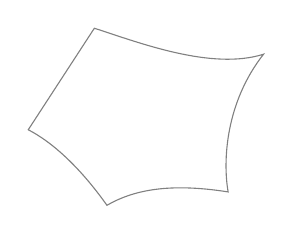
\begin{tikzpicture}[x=.01cm,y=-.01cm]
\draw[gray] (2374,817)..controls(2430,835)and(2523,871)..(2589,850)..controls(2541,911)and(2537,985)..(2544,1025)..controls(2468,1013)and(2423,1023)..(2390,1042)..controls(2356,994)and(2321,962)..(2290,946)--cycle;
\end{tikzpicture}}
\margin{\[\overbrace{\unsure{\tau_s|\sigma_s}\quad\unsure{\tau_a|\sigma_a}}\quad\unsure{\tau_r|\sigma_r}\qquad\unsure{\tau_{\deleted{\unsure{ver}}t}|\sigma_t}\]}
\figure{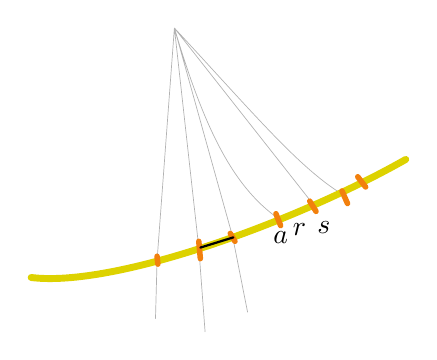
\begin{tikzpicture}[x=.01cm,y=-.01cm,line cap=round]
\draw[gray!60,line width=.25pt] (2457,1114)--(2435,1409)--(2433,1483) (2457,1114)--(2488,1393)--(2496,1500) (2457,1114)--(2531,1379)--(2550,1475) (2457,1114)..controls(2493,1235)and(2529,1314)..(2589,1356) (2457,1114)--(2635,1340) (2457,1114)..controls(2560,1225)and(2618,1295)..(2675,1328);
\draw[yellow!70!olive,line width=2.5pt] (2275,1431)..controls(2380,1444)and(2610,1361)..(2751,1281);
\draw[orange!80!brown,line width=2pt] (2435,1404)--(2436,1414) (2488,1385)--(2490,1407) (2528,1375)--(2534,1385) (2586,1350)--(2592,1365) (2629,1334)--(2637,1347) (2670,1321)--(2677,1337) (2690,1303)--(2700,1316);
\draw[line width=.8pt] (2490,1393)--(2532,1380);
\node at (2592,1380) {$a$};\node at (2616,1370) {$r$};\node at (2647,1368) {$s$};
\end{tikzpicture}}
\margin{94}
